\documentclass[10pt, twocolumn]{article}

% packages
\usepackage[margin=1in]{geometry}
\usepackage[utf8]{inputenc}
\usepackage{hyperref}
\usepackage{graphicx}
\usepackage{mathptmx}
\usepackage[none]{hyphenat}
\usepackage{titlesec}

% parameters
\setlength{\parskip}{0.6em}
\hypersetup{colorlinks=true, urlcolor=blue}
\graphicspath{{./img/}}
\titlespacing{\section}{6pt}{\parskip}{0.5em}
\titlespacing{\subsection}{6pt}{\parskip}{0.2em}
\titlespacing{\subsubsection}{6pt}{\parskip}{0.1em}

\title{\textbf{Listen to drivers: How Uber drivers organize through a forum}}
\author{authors\footnote{Department of Civil Engineering, Purdue University, West Lafayette, IN 47906}}
\date{February 2020}

\begin{document}

\maketitle

\section{Introduction}

\subsection{Background}
Uber\texttrademark was created in March 2009 with the objective of reducing the cost of on-demand private road transportation. As a ride-hailing company, its core business involves providing a platform for passengers to match rides with automobile drivers associated with the service. The company is also different from the conventional taxicab system in that it does not own or maintain the vehicle fleet it helps operate. 

Uber drivers drive vehicles they own or rent privately, set their own driving work schedule, and earn on a per-trip basis based on dynamic fares calculated by the service that depend on various factors. This contractual and part-time nature of work also allows them to engage in other professions, including driving for other ride-hailing services. This complicates the drivers' employment status and relationship with the company. Officially, Uber drivers are considered independent contractors instead of formal employees of the company, making them ineligible for benefits like expense compensation, minimum wages, health care benefits as well as unionization.

Uber, like other ridehailing companies, has also been criticized on various occasions for unfair treatment to drivers, exercise of inadequate and non-uniform regulations, and aggressive opposition to government regulations. On January 1, 2020, the senate of California, the state where Uber is incorporated, passed Assembly Bill 5 which mandates considering these drivers as employees and therefore entitled to employee benefits. This legislation came into effect after public discussions followed by strikes staged by Uber and Lyft\texttrademark drivers across the U.S. in September 2019, but is currently being contested by both Uber and Lyft.

\subsubsection{UberPeople}
Since drivers are and have not been legally allowed to unionize and demand employee rights, they have resorted to organize on independent platforms such as social media groups and online forums. One such discussion forum is ``\href{https://uberpeople.net/}{UberPeople}" which was formed in April, 2014. It allows them to create and participate in discussion threads across different categories and places in the U.S. As of February 28, 2020, it has $\sim$150,000 members who have created $\sim$340,000 threads containing a total of $\sim$5.6 million messages.

\begin{figure}
    \centering
    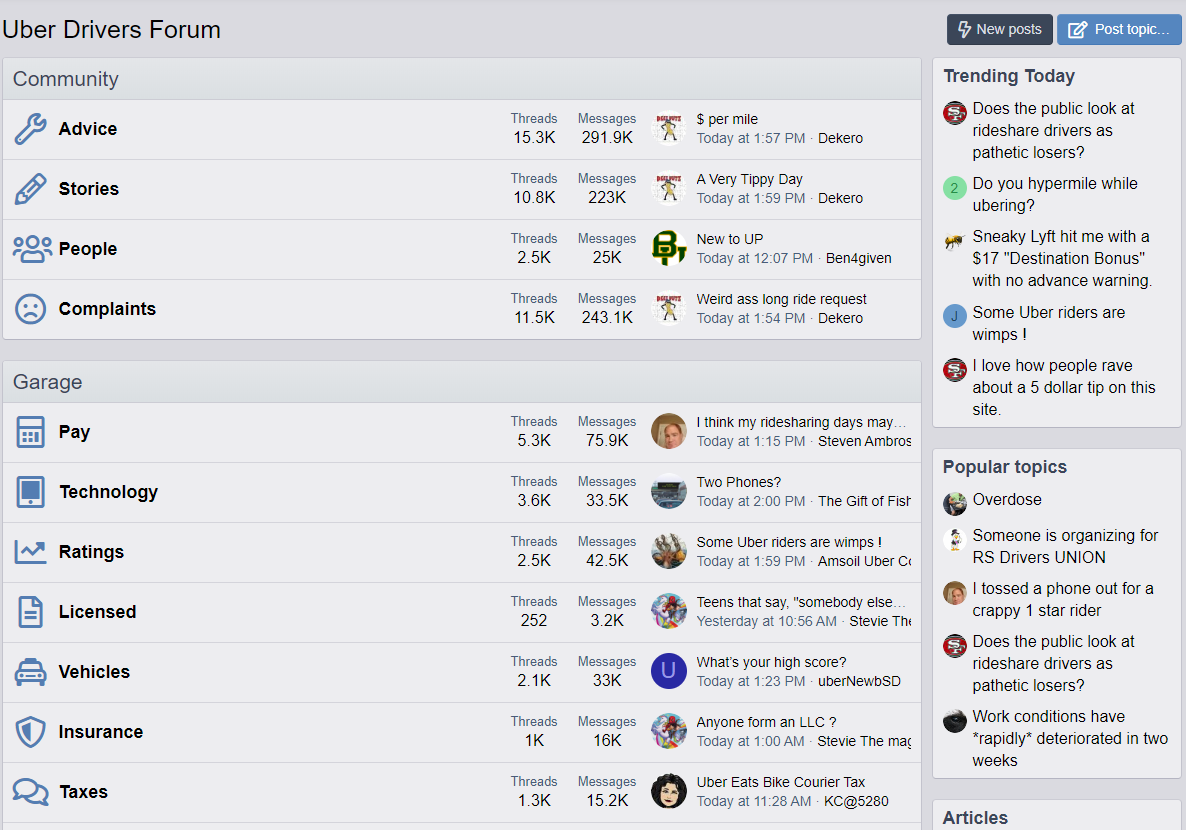
\includegraphics[width=0.45\textwidth]{img/home-screen-sample.png}
    \caption{Screenshot of the UberPeople homepage}
    \label{fig:home-screen-sample}
\end{figure}

\subsection{Problem Description and Objectives}
Our preliminary understanding is that in the absence of a union, Uber drivers have used multiple platforms for organizing, including social media (e.g. Facebook, Twitter) and online forums, principally UberPeople. In this study, our broad objective is to:
\begin{enumerate}
    \item find the mechanism of information sharing within the driver community active on UberPeople,
    \item quantify the effectiveness of this forum in helping them organize and exert public pressure for employee rights and better working conditions for themselves.
\end{enumerate}
We attempt to do this by studying the social network involved in this forum community as well as the qualitative properties of the content they post. In particular, we attempt to answer the following questions based on the contents of this forum:
\begin{enumerate}
    \item How have the topics discussed in this community changed over time in relation to Uber's policies and the corresponding socio-political environment?
    \item What was the role of the structure of the social network within this forum in influencing the driver strikes of 2015 and 2019? How can this structure be improved by artificial means to maximize the effectiveness of this forum for organizing?
\end{enumerate}

\section{Literature Review}

\section{Data Description}

\begin{figure}[b]
    \centering
    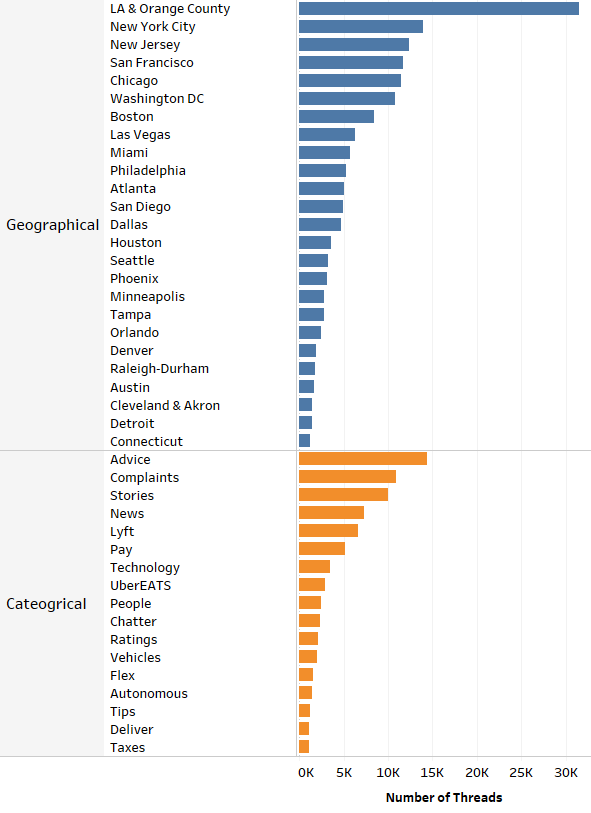
\includegraphics[width=0.45\textwidth]{img/Threads by Forum.png}
    \caption{Distribution of threads across categories}
    \label{fig:threads-by-forum}
\end{figure}

\section{Methodology}

\section{Observations}

\end{document}
